%!TEX root = ../polycat.tex

\begin{frame}[fragile]{Polytopes}
	\pause
	A \colorit{polytope} $P$ is the convex closure of a finite number of points in $\R^n$.
	\smallskip
	\begin{center}
		\includegraphics[scale=.15]{aux/random_polytope}
	\end{center}

	\vskip-10pt\pause
	Its faces form a poset $\colorit{\faces(P)}$:
	\[
	F \leq G \qquad iff \qquad F \subseteq G.
	\]

	\pause\medskip

	The \colorit{linear span} of $F \in \faces(P)$ is denoted $\colorit{\Lin F}$.
\end{frame}

\begin{frame}{Oriented polytopes}
	\pause

	Let $V$ be an $n$-dim'l vector space.

	\medskip
	Two ordered bases define the same \colorit{orientation} $\omega$ if they are related by a positive determinant $\lambda$:
	\[
	v_1 \wedge\dots\wedge v_n = \lambda \ w_1 \wedge\dots\wedge w_n
	\]

	\pause\medskip
	An \colorit{oriented polytope} is:
	 \begin{enumerate}
	 	\item A polytope $P$ and
	 	\item $\forall F \in \faces(P)$ an orientation $\omega_F$ of $\Lin F$.
	 \end{enumerate}
\end{frame}

\begin{frame}[fragile]{Frames}
	\pause
	A \colorit{frame} is an ordered basis $\set{v_i}$ of $\R^n$:
	\begin{center}
		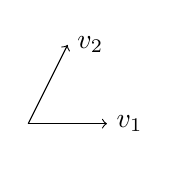
\begin{tikzpicture}
			\draw[->] (2, 0) -- (3, 0) node[anchor=west]{$v_1$};
			\draw[->] (2, 0) -- (2.5, 1) node[anchor=west]{$v_2$};
		\end{tikzpicture}
	\end{center}

	\pause
	It defines a filtration: \quad $0 = V_0 \leq V_1 \leq\dots\leq V_n = \R^n$
	\[
	V_k = \Span{(v_1,\ldots,v_k)}
	\]
%	\[
%	V_0 \leq V_1 \leq\dots\leq V_n = \R^n
%	\]

	\pause\medskip
	Its \colorit{system of projections} is the collection
	\[
	\set{\pi_k \colon \R^n \to V_k}
	\quad ; \quad
	\pi_k(v_i) =
	\begin{cases}
		v_i & i \leq k,\\
		\hfil 0 & k > i.
	\end{cases}
	\]
\end{frame}

\begin{frame}[fragile]{Framed polytopes}
	\pause
	A frame is said to be \colorit{$P$-admissible} if
	\[
	\forall F \in \faces(P),\ \pi_{\dim F}(\Lin F) = V_{\dim F}.
	\]
	We denote its inverse by $\sigma_F$.

	\medskip
	\colorit{Example}
	\begin{center}
		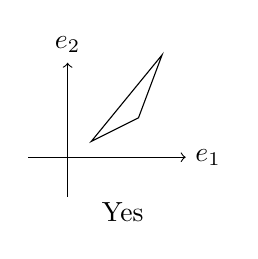
\begin{tikzpicture}
			% Draw edges
			\draw (.3,.2) -- (.9,.5) -- (1.2,1.3) -- cycle;

			% Draw axes
			\draw[->] (-0.5,0) -- (1.5,0) node[right] {$e_1$};
			\draw[->] (0,-0.5) -- (0,1.2) node[above] {$e_2$};

			\node at (.7,-.7){Yes};
		\end{tikzpicture}
		\qquad\qquad
		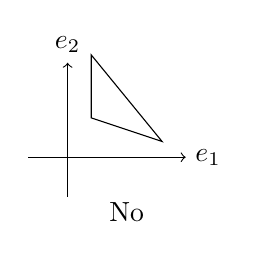
\begin{tikzpicture}
			% Draw edges
			\draw (1.2,.2) -- (.3,.5) -- (.3,1.3) -- cycle;

			% Draw axes
			\draw[->] (-0.5,0) -- (1.5,0) node[right] {$e_1$};
			\draw[->] (0,-0.5) -- (0,1.2) node[above] {$e_2$};

			\node at (.7,-.7){\;No};
		\end{tikzpicture}
	\end{center}

	\pause\medskip
	A \colorit{framed polytope} is
	\begin{enumerate}
		\item A polytope $P$ and
		\item A $P$-admissible frame $\set{v_i}$.
	\end{enumerate}
\end{frame}

\begin{frame}{Orientation from frame}
	\pause
	\colorit{Construction} A $P$-admissible frame $\{v_i\}$ determines an orientation of $P$\,:
	\[
	\forall F \in \faces(P), \ \omega_F = \sigma_F v_1 \wedge\dots\wedge \sigma_F v_{\dim F}.
	\]

	\pause\colorit{Questions}
	\begin{enumerate}
		\item What frames induce the same orientation?
		\item What orientations come from frames?
	\end{enumerate}
\end{frame}

\begin{frame}{Frames over an orientation}
	\pause
	The \colorit{frame moduli} of an orientation $\omega$ of $P$ is the set $\mathcal{M}(\omega)$ of all $P$-admissible frames inducing $\omega$.

	\pause
	\begin{center}
		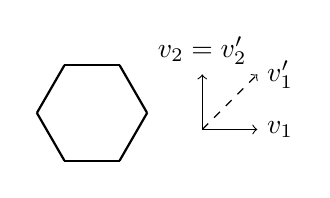
\begin{tikzpicture}[scale=.7]
		%axes
		\draw[->] (2, -.3) -- (3, -.3) node[anchor=west]{$v_1$};
		\draw[->,dashed] (2, -.3) -- (3, .7) node[anchor=west]{$v_1'$};
		\draw[->] (2, -.3) -- (2, .7) node[anchor=south]{$v_2=v_2'$};

		%vertices
		\node (a) at (1, 0) {};
		%\node at (1.3, 0) {$a$};

		\node (b) at (0.5, 0.866) {};
		%\node at (0.5, 1.2) {$b$};

		\node (c) at (-0.5, 0.866) {};
		%\node (c) at (-0.5, 1.2) {$c$};

		\node (d) at (-1, 0) {};
		%\node at (-1.3, 0) {$d$};

		\node (e) at (-0.5, -0.866) {};
		%\node at (-0.5, -1.2) {$e$};

		\node (f) at (0.5, -0.866) {};
		%\node at (0.5, -1.2) {$f$};

		%upper dges
		\draw[thick] (-0.5, 0.866)--(0.5, 0.866);
		\draw[thick] (1, 0)--(0.5, 0.866);
		\draw[thick] (-0.5, 0.866)--(-1, 0);

		%lower edges
		\draw[thick] (1,0)--(0.5, -0.866);
		\draw[thick] (-0.5, -0.866)--(0.5, -0.866);
		\draw[thick] (-0.5, -0.866)--(-1, 0) ;
	\end{tikzpicture}
	\end{center}

	\pause\medskip
	\alt<4>{\colorit{Question} How complicated can this moduli be?}{
	A \colorit{semi-algebraic set} $S \subseteq \R^d$ is def'd by integral poly. eqs. and inequalities
	\[
	S = \set{\mathbf{x}\in\R^d \mid f_1(\mathbf{x})=0, \dots, f_k(\mathbf{x})=0, f_{k+1}(\mathbf{x})>0, \dots, f_r(\mathbf{x})>0}.
	\]
	}
	\pause
	An important relation $\sim_{\mathrm{st}}$ between them is \colorit{stable equivalence}.

	\pause\bigskip
	\colorit{Universality Theorem (LPM)}
	For any open semi-algebraic set $S$ there exist $n \in \N$ and an orientation $\omega$ of the $n$-simplex with $\cM(\omega) \sim_{\mathrm{st}} S$.
\end{frame}

\begin{frame}[fragile]{Pasting diagrams}
	\pause

	\colorit{Construction} The category $F(G)$ generated by a directed graph $G$.

	\pause\medskip
	\colorit{Roughly} $G$ is a \colorit{pasting diagram} if each morphism in $F(G)$ is uniquely expressible in diagramatical terms.
	For example,
	\[
	\cdot \to \cdot \to \cdot \to \dots \to \cdot
	\qquad\text{but not}\qquad
	\begin{tikzcd}[column sep=9pt,row sep=9pt]
		\arrow[d,<-] \arrow[r] \cdot & \arrow[d] \cdot \\
		\arrow[r,,<-] \cdot & \cdot
	\end{tikzcd}
	\]

	\pause
	Similarly, in higher category theory, this is a pasting diagram
	\medskip
	\begin{center}
		% !TEX root = ../tqft.tex

\tikzstyle{object} = [circle, fill, minimum size=2pt, inner sep=0pt, outer sep=0pt]

\begin{tikzpicture}[auto, node distance=2cm,>=latex']
	\node[object] (0) {};
	\node[object] (1) at (1,1) {};
	\node[object] (2) at (3,1) {};
	\node[object] (3) at (4,0) {};
	\node[object] (4) at (5,0) {};
	\node[object] (5) at (6.5,0) {};
	\node[object] (6) at (8,1) {};
	\node[object] (7) at (9,0) {};

	\draw[->]
	(0) edge (1)
	(1) edge (2)
	(2) edge (3)
	(3) edge (4);

	\draw[->] (4) to[out=90,in=90] (5);
	\draw[->] (4) to[out=-90,in=-90] (5);

	\draw[->]
	(5) edge (6)
	(6) edge (7)
	(5) edge (7);

	\node[object] (21) at (1,-1) {};
	\node[object] (22) at (3,-1) {};

	\draw[->]
	(0) edge (21)
	(21) edge (22)
	(22) edge (3);

	\node[object] (8) at (2,0) {};
	\draw[->]
	(0) edge (8)
	(8) edge (2)
	(8) edge (22);

	\node at (1.5,.5){$\Downarrow$};
	\node at (1.5,-.5){$\Downarrow$};
	\node at (3,0){$\Downarrow$};
	\node at (5.8,0){$\Downarrow$};
	\node at (8,.4){$\Downarrow$};
\end{tikzpicture}
	\end{center}

	\pause\smallskip
	\colorit{Conjecture (Kapranov-Voevodsky)}

	\smallskip
	Every framed polytope defines a pasting diagram.
\end{frame}

\begin{frame}{Simplices as pasting diagrams (Street 1987)}
	\pause
	\begin{center}
		\includegraphics[scale=.28]{aux/street}
	\end{center}
\end{frame}

\begin{frame}{Continued}
	\vspace*{-10pt}
	\begin{center}
		\includegraphics[scale=.25]{aux/street2}
	\end{center}
\end{frame}

\begin{frame}{Digression (for homotopy theorist)}
	\pause
	Street's construction defines a functor
	\[
	\simplex \to \infty\Cat
	\]
	\pause
	and, given that the target is cocomplete, also the nerve of higher cats
	\[
	\rN \colon \infty\Cat \to \sSet
	\]
	whose image is used to define weak $\infty$-cats (complicial sets).

	\pause\bigskip
	\colorit{Disclaimer} This will play no role today.

	\pause\bigskip
	Let us go back to the idea of Kapranov-Voevodsky.
\end{frame}

\begin{frame}{Sources and targets}
	\pause
	Let $P$ be framed by $\{v_i\}$ and $F \in \faces(P)$.

	\medskip
	For $k < \dim F$, the \colorit{$k$-boundary} $\bd^{(k)}(F)$ is the boundary of $\pi_{k+1}(F)$.

	\pause\smallskip
	It has a canonical splitting:
	\[
	\bd^{(k)}(F) = \colorit{\so_k(F)} \sqcup \colorit{\ta_k(F)}
	\]
	where these are defined using the normal
	\[
	\angles{\normal, v_{k+1}} < 0 \quad (\text{resp.} > 0).
	\]

	\pause\medskip
	\colorit{Example} ...
\end{frame}

\begin{frame}{Example}
	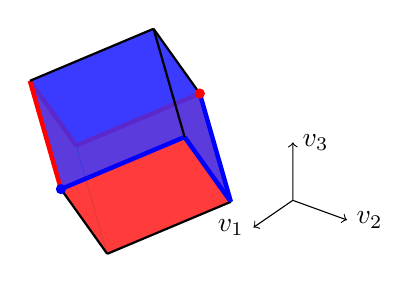
\begin{tikzpicture}%
	[x={(-0.587802cm, -0.404450cm)},
	y={(0.809005cm, -0.293947cm)},
	z={(0.000078cm, 0.866034cm)},
	scale=.850000,
	back/.style={thin, color=black!60},
	edge/.style={color=black, thick},
	sourceedge/.style={color=red, ultra thick},
	targetedge/.style={color=blue, ultra thick},
	facet/.style={fill=blue!95!black,fill opacity=0.800000},
	targetfacet/.style={fill=blue!80,fill opacity=0.800000},
	sourcefacet/.style={fill=red!80,fill opacity=0.800000},
	vertex/.style={inner sep=1pt,circle,draw=black,fill=black,thick},
	targetvertex/.style={inner sep=1pt,circle,draw=blue,fill=blue,thick},
	sourcevertex/.style={inner sep=1pt,circle,draw=red,fill=red,thick}]
	%
	%
	%% This TikZ-picture was produced with Sagemath version 10.0
	%% with the command: ._tikz_3d_in_3d and parameters:
	%% view = [-0.246900000000000, -0.484500000000000, -0.839200000000000]
	%% angle = 133.700000000000
	%% scale = 1
	%% edge_color = blue!95!black
	%% facet_color = blue!95!black
	%% opacity = 0.8
	%% vertex_color = green
	%% axis = False
	%%
	%% Coordinate of the vertices:
	%%
	\coordinate (-0.58824, 1.42857, -0.83333) at (-0.58824, 1.42857, -0.83333);
	\coordinate (0.58824, 1.42857, 0.83333) at (0.58824, 1.42857, 0.83333);
	\coordinate (1.76471, 0.00000, 0.00000) at (1.76471, 0.00000, 0.00000);
	\coordinate (0.58824, 0.00000, -1.66667) at (0.58824, 0.00000, -1.66667);
	\coordinate (-0.58824, -1.42857, -0.83333) at (-0.58824, -1.42857, -0.83333);
	\coordinate (-1.76471, 0.00000, 0.00000) at (-1.76471, 0.00000, 0.00000);
	\coordinate (-0.58824, 0.00000, 1.66667) at (-0.58824, 0.00000, 1.66667);
	\coordinate (0.58824, -1.42857, 0.83333) at (0.58824, -1.42857, 0.83333);
	%%
	%%
	%% Drawing edges in the back
	%%

	%%
	%%
	%% Drawing vertices in the back
	%%
	% \node[vertex] at (-0.58824, -1.42857, -0.83333)     {};
	%%
	%%
	\fill[targetfacet] (-0.58824, 0.00000, 1.66667) -- (0.58824, -1.42857, 0.83333) -- (-0.58824, -1.42857, -0.83333) -- (-1.76471, 0.00000, 0.00000) -- cycle {};
	\fill[sourcefacet] (-0.58824, 1.42857, -0.83333) -- (-1.76471, 0.00000, 0.00000) -- (-0.58824, -1.42857, -0.83333) -- (0.58824, 0.00000, -1.66667) -- cycle {};
	\fill[sourcefacet] (0.58824, 0.00000, -1.66667) -- (-0.58824, -1.42857, -0.83333) -- (0.58824, -1.42857, 0.83333) -- (1.76471, 0.00000, 0.00000) -- cycle {};


	\draw[edge,back] (0.58824, 0.00000, -1.66667) -- (-0.58824, -1.42857, -0.83333);
	\draw[back,sourceedge] (-0.58824, -1.42857, -0.83333) -- (-1.76471, 0.00000, 0.00000);
	\draw[back,sourceedge] (-0.58824, -1.42857, -0.83333) -- (0.58824, -1.42857, 0.83333);

	% %% Drawing the facets
	% %%
	\fill[sourcefacet] (0.58824, 0.00000, -1.66667) -- (-0.58824, 1.42857, -0.83333) -- (0.58824, 1.42857, 0.83333) -- (1.76471, 0.00000, 0.00000) -- cycle {};
	\fill[targetfacet] (0.58824, -1.42857, 0.83333) -- (1.76471, 0.00000, 0.00000) -- (0.58824, 1.42857, 0.83333) -- (-0.58824, 0.00000, 1.66667) -- cycle {};
	\fill[targetfacet] (-0.58824, 0.00000, 1.66667) -- (0.58824, 1.42857, 0.83333) -- (-0.58824, 1.42857, -0.83333) -- (-1.76471, 0.00000, 0.00000) -- cycle {};
	%%
	%%
	%% Drawing edges in the front
	%%
	\draw[targetedge] (-0.58824, 1.42857, -0.83333) -- (0.58824, 1.42857, 0.83333);
	\draw[edge] (-0.58824, 1.42857, -0.83333) -- (0.58824, 0.00000, -1.66667);
	\draw[targetedge] (-0.58824, 1.42857, -0.83333) -- (-1.76471, 0.00000, 0.00000);
	\draw[targetedge] (0.58824, 1.42857, 0.83333) -- (1.76471, 0.00000, 0.00000);
	\draw[edge] (0.58824, 1.42857, 0.83333) -- (-0.58824, 0.00000, 1.66667);
	\draw[edge] (1.76471, 0.00000, 0.00000) -- (0.58824, 0.00000, -1.66667);
	\draw[sourceedge] (1.76471, 0.00000, 0.00000) -- (0.58824, -1.42857, 0.83333);
	\draw[edge] (-1.76471, 0.00000, 0.00000) -- (-0.58824, 0.00000, 1.66667);
	\draw[edge] (-0.58824, 0.00000, 1.66667) -- (0.58824, -1.42857, 0.83333);
	%%
	%%
	% %% Drawing the vertices in the front
	% %%
	% \node[vertex] at (-0.58824, 1.42857, -0.83333)     {};
	% \node[vertex] at (0.58824, 1.42857, 0.83333)     {};
	\node[targetvertex] at (1.76471, 0.00000, 0.00000)     {};
	% \node[vertex] at (0.58824, 0.00000, -1.66667)     {};
	\node[sourcevertex] at (-1.76471, 0.00000, 0.00000)     {};
	% \node[vertex] at (-0.58824, 0.00000, 1.66667)     {};
	% \node[vertex] at (0.58824, -1.42857, 0.83333)     {};
	% %%
	% %%
	% %
	\begin{scope}[shift={(0,3,0)}]

		%axes
		\draw[->] (0, 0,0) -- (1, 0,0) node[anchor=east]{$v_1$};
		\draw[->] (0, 0,0) -- (0, 1,0) node[anchor=west]{$v_2$};
		\draw[->] (0, 0,0) -- (0, 0, 1) node[anchor=west]{$v_3$};
	\end{scope}

\end{tikzpicture}
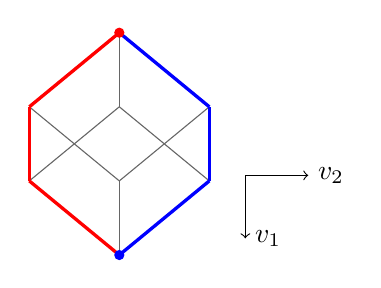
\begin{tikzpicture}%
	[
	x={(0.000000cm, -1.000000cm)},
	y={(1.000000cm, 0.000000cm)},
	z={(0.000000cm, 0.000000cm)},
	scale=.8,
	back/.style={thin, color=black!60},
	edge/.style={color=black, thick},
	sourceedge/.style={color=red, very thick},
	targetedge/.style={color=blue, very thick},
	facet/.style={fill=blue!95!black,fill opacity=0.800000},
	targetfacet/.style={fill=blue,fill opacity=0.600000},
	sourcefacet/.style={fill=red,fill opacity=0.600000},
	vertex/.style={inner sep=1pt,circle,draw=black,fill=black,thick},
	targetvertex/.style={inner sep=1pt,circle,draw=blue,fill=blue,thick},
	sourcevertex/.style={inner sep=1pt,circle,draw=red,fill=red,thick}]

\coordinate (-0.58824, 1.42857, -0.83333) at (-0.58824, 1.42857, -0.83333);
\coordinate (0.58824, 1.42857, 0.83333) at (0.58824, 1.42857, 0.83333);
\coordinate (1.76471, 0.00000, 0.00000) at (1.76471, 0.00000, 0.00000);
\coordinate (0.58824, 0.00000, -1.66667) at (0.58824, 0.00000, -1.66667);
\coordinate (-0.58824, -1.42857, -0.83333) at (-0.58824, -1.42857, -0.83333);
\coordinate (-1.76471, 0.00000, 0.00000) at (-1.76471, 0.00000, 0.00000);
\coordinate (-0.58824, 0.00000, 1.66667) at (-0.58824, 0.00000, 1.66667);
\coordinate (0.58824, -1.42857, 0.83333) at (0.58824, -1.42857, 0.83333);

\draw[edge,back] (-0.58824, 1.42857, -0.83333) -- (0.58824, 0.00000, -1.66667);
\draw[edge,back] (1.76471, 0.00000, 0.00000) -- (0.58824, 0.00000, -1.66667);
\draw[edge,back] (0.58824, 0.00000, -1.66667) -- (-0.58824, -1.42857, -0.83333);

\draw[edge,back] (0.58824, 1.42857, 0.83333) -- (-0.58824, 0.00000, 1.66667);
\draw[edge,back] (-1.76471, 0.00000, 0.00000) -- (-0.58824, 0.00000, 1.66667);
\draw[edge,back] (-0.58824, 0.00000, 1.66667) -- (0.58824, -1.42857, 0.83333);

\draw[back,sourceedge] (-0.58824, -1.42857, -0.83333) -- (-1.76471, 0.00000, 0.00000);
\draw[back,sourceedge] (-0.58824, -1.42857, -0.83333) -- (0.58824, -1.42857, 0.83333);
\draw[targetedge] (-0.58824, 1.42857, -0.83333) -- (0.58824, 1.42857, 0.83333);
\draw[targetedge] (-0.58824, 1.42857, -0.83333) -- (-1.76471, 0.00000, 0.00000);
\draw[targetedge] (0.58824, 1.42857, 0.83333) -- (1.76471, 0.00000, 0.00000);
\draw[sourceedge] (1.76471, 0.00000, 0.00000) -- (0.58824, -1.42857, 0.83333);
\node[targetvertex] at (1.76471, 0.00000, 0.00000)     {};
\node[sourcevertex] at (-1.76471, 0.00000, 0.00000)     {};
\begin{scope}[shift={(.5,2,0)}]
	\draw[->] (0, 0,0) -- (1, 0,0) node[anchor=west]{$v_1$};
	\draw[->] (0, 0,0) -- (0, 1,0) node[anchor=west]{$v_2$};
\end{scope}
\end{tikzpicture}
\begin{tikzpicture}%
	[scale=.8,
	back/.style={thin, color=black!60},
	edge/.style={color=black, thick},
	sourceedge/.style={color=red, very thick},
	targetedge/.style={color=blue, very thick},
	facet/.style={fill=blue!95!black,fill opacity=0.800000},
	targetfacet/.style={fill=blue,fill opacity=0.600000},
	sourcefacet/.style={fill=red,fill opacity=0.600000},
	vertex/.style={inner sep=1pt,circle,draw=black,fill=black,thick},
	targetvertex/.style={inner sep=1pt,circle,draw=blue,fill=blue,thick},
	sourcevertex/.style={inner sep=1pt,circle,draw=red,fill=red,thick}]
	\draw[edge] (0,-2) -- (0,1);
	\node[targetvertex] at (0,-2)     {};
	\node[sourcevertex] at (0,1)     {};

	\begin{scope}[shift={(1,-1)}]
		%axes
		\draw[->] (0, 0) -- ( 0,-1) node[anchor=west]{$v_1$};
	\end{scope}
\end{tikzpicture}
\vspace*{.8cm}

\pause
\centering
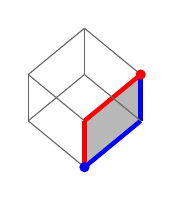
\begin{tikzpicture}%
	[	x={(0.000000cm, -1.000000cm)},
	y={(1.000000cm, 0.000000cm)},
	z={(0.000000cm, 0.000000cm)},
	scale=.5,
	back/.style={thin, color=black!60},
	edge/.style={color=black!60, thin},
	sourceedge/.style={color=red, ultra thick},
	targetedge/.style={color=blue, ultra thick},
	facet/.style={fill=black!35,fill opacity=0.800000},
	targetfacet/.style={fill=blue!80,fill opacity=0.800000},
	sourcefacet/.style={fill=red!80,fill opacity=0.800000},
	vertex/.style={inner sep=1pt,circle,draw=black,fill=black,thick},
	targetvertex/.style={inner sep=1pt,circle,draw=blue,fill=blue,thick},
	sourcevertex/.style={inner sep=1pt,circle,draw=red,fill=red,thick}]

\coordinate (-0.58824, 1.42857, -0.83333) at (-0.58824, 1.42857, -0.83333);
\coordinate (0.58824, 1.42857, 0.83333) at (0.58824, 1.42857, 0.83333);
\coordinate (1.76471, 0.00000, 0.00000) at (1.76471, 0.00000, 0.00000);
\coordinate (0.58824, 0.00000, -1.66667) at (0.58824, 0.00000, -1.66667);
\coordinate (-0.58824, -1.42857, -0.83333) at (-0.58824, -1.42857, -0.83333);
\coordinate (-1.76471, 0.00000, 0.00000) at (-1.76471, 0.00000, 0.00000);
\coordinate (-0.58824, 0.00000, 1.66667) at (-0.58824, 0.00000, 1.66667);
\coordinate (0.58824, -1.42857, 0.83333) at (0.58824, -1.42857, 0.83333);

\draw[edge,back] (0.58824, 0.00000, -1.66667) -- (-0.58824, -1.42857, -0.83333);
\draw[edge,back] (-0.58824, -1.42857, -0.83333) -- (-1.76471, 0.00000, 0.00000);
\draw[edge,back] (-0.58824, -1.42857, -0.83333) -- (0.58824, -1.42857, 0.83333);

\fill[facet] (0.58824, 0.00000, -1.66667) -- (-0.58824, 1.42857, -0.83333) -- (0.58824, 1.42857, 0.83333) -- (1.76471, 0.00000, 0.00000) -- cycle {};

\draw[targetedge] (-0.58824, 1.42857, -0.83333) -- (0.58824, 1.42857, 0.83333);
\draw[sourceedge] (-0.58824, 1.42857, -0.83333) -- (0.58824, 0.00000, -1.66667);
\draw[edge] (-0.58824, 1.42857, -0.83333) -- (-1.76471, 0.00000, 0.00000);
\draw[targetedge] (0.58824, 1.42857, 0.83333) -- (1.76471, 0.00000, 0.00000);
\draw[edge] (0.58824, 1.42857, 0.83333) -- (-0.58824, 0.00000, 1.66667);
\draw[sourceedge] (1.76471, 0.00000, 0.00000) -- (0.58824, 0.00000, -1.66667);
\draw[edge] (1.76471, 0.00000, 0.00000) -- (0.58824, -1.42857, 0.83333);
\draw[edge] (-1.76471, 0.00000, 0.00000) -- (-0.58824, 0.00000, 1.66667);
\draw[edge] (-0.58824, 0.00000, 1.66667) -- (0.58824, -1.42857, 0.83333);

\node[sourcevertex] at (-0.58824, 1.42857, -0.83333)     {};
\node[targetvertex] at (1.76471, 0.00000, 0.00000)     {};
\end{tikzpicture}
\qquad
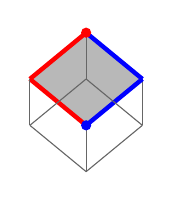
\begin{tikzpicture}%
	[x={(0.000000cm, -1.000000cm)},
	y={(1.000000cm, 0.000000cm)},
	z={(0.000000cm, 0.000000cm)},,
	scale=.5,
	back/.style={thin, color=black!60},
	edge/.style={color=black!60, thin},
	sourceedge/.style={color=red, ultra thick},
	targetedge/.style={color=blue, ultra thick},
	facet/.style={fill=black!35,fill opacity=0.800000},
	targetfacet/.style={fill=blue!80,fill opacity=0.800000},
	sourcefacet/.style={fill=red!80,fill opacity=0.800000},
	vertex/.style={inner sep=1pt,circle,draw=black,fill=black,thick},
	targetvertex/.style={inner sep=1pt,circle,draw=blue,fill=blue,thick},
	sourcevertex/.style={inner sep=1pt,circle,draw=red,fill=red,thick}]
%
\coordinate (-0.58824, 1.42857, -0.83333) at (-0.58824, 1.42857, -0.83333);
\coordinate (0.58824, 1.42857, 0.83333) at (0.58824, 1.42857, 0.83333);
\coordinate (1.76471, 0.00000, 0.00000) at (1.76471, 0.00000, 0.00000);
\coordinate (0.58824, 0.00000, -1.66667) at (0.58824, 0.00000, -1.66667);
\coordinate (-0.58824, -1.42857, -0.83333) at (-0.58824, -1.42857, -0.83333);
\coordinate (-1.76471, 0.00000, 0.00000) at (-1.76471, 0.00000, 0.00000);
\coordinate (-0.58824, 0.00000, 1.66667) at (-0.58824, 0.00000, 1.66667);
\coordinate (0.58824, -1.42857, 0.83333) at (0.58824, -1.42857, 0.83333);
%%
%%
%% Drawing edges in the back
%%

%%
%%
%% Drawing vertices in the back
%%
% \node[vertex] at (-0.58824, -1.42857, -0.83333)     {};
%%
%%
% \fill[targetfacet] (-0.58824, 0.00000, 1.66667) -- (0.58824, -1.42857, 0.83333) -- (-0.58824, -1.42857, -0.83333) -- (-1.76471, 0.00000, 0.00000) -- cycle {};
\fill[facet] (-0.58824, 1.42857, -0.83333) -- (-1.76471, 0.00000, 0.00000) -- (-0.58824, -1.42857, -0.83333) -- (0.58824, 0.00000, -1.66667) -- cycle {};
%  \fill[sourcefacet] (0.58824, 0.00000, -1.66667) -- (-0.58824, -1.42857, -0.83333) -- (0.58824, -1.42857, 0.83333) -- (1.76471, 0.00000, 0.00000) -- cycle {};


\draw[back,sourceedge] (0.58824, 0.00000, -1.66667) -- (-0.58824, -1.42857, -0.83333);
\draw[back,sourceedge] (-0.58824, -1.42857, -0.83333) -- (-1.76471, 0.00000, 0.00000);
\draw[edge,back] (-0.58824, -1.42857, -0.83333) -- (0.58824, -1.42857, 0.83333);

% %% Drawing the facets
% %%
% \fill[facet] (0.58824, 0.00000, -1.66667) -- (-0.58824, 1.42857, -0.83333) -- (0.58824, 1.42857, 0.83333) -- (1.76471, 0.00000, 0.00000) -- cycle {};
% \fill[facet] (0.58824, -1.42857, 0.83333) -- (1.76471, 0.00000, 0.00000) -- (0.58824, 1.42857, 0.83333) -- (-0.58824, 0.00000, 1.66667) -- cycle {};
%  \fill[targetfacet] (-0.58824, 0.00000, 1.66667) -- (0.58824, 1.42857, 0.83333) -- (-0.58824, 1.42857, -0.83333) -- (-1.76471, 0.00000, 0.00000) -- cycle {};
%%
%%
%% Drawing edges in the front
%%
\draw[edge] (-0.58824, 1.42857, -0.83333) -- (0.58824, 1.42857, 0.83333);
\draw[targetedge] (-0.58824, 1.42857, -0.83333) -- (0.58824, 0.00000, -1.66667);
\draw[targetedge] (-0.58824, 1.42857, -0.83333) -- (-1.76471, 0.00000, 0.00000);
\draw[edge] (0.58824, 1.42857, 0.83333) -- (1.76471, 0.00000, 0.00000);
\draw[edge] (0.58824, 1.42857, 0.83333) -- (-0.58824, 0.00000, 1.66667);
\draw[edge] (1.76471, 0.00000, 0.00000) -- (0.58824, 0.00000, -1.66667);
\draw[edge] (1.76471, 0.00000, 0.00000) -- (0.58824, -1.42857, 0.83333);
\draw[edge] (-1.76471, 0.00000, 0.00000) -- (-0.58824, 0.00000, 1.66667);
\draw[edge] (-0.58824, 0.00000, 1.66667) -- (0.58824, -1.42857, 0.83333);
%%
%%
% %% Drawing the vertices in the front
% %%
% \node[vertex] at (-0.58824, 1.42857, -0.83333)     {};
% \node[targetvertex] at (0.58824, 1.42857, 0.83333)     {};
% \node[targetvertex] at (1.76471, 0.00000, 0.00000)     {};
 \node[targetvertex] at (0.58824, 0.00000, -1.66667)     {};
 \node[sourcevertex] at (-1.76471, 0.00000, 0.00000)     {};
% \node[vertex] at (-0.58824, 0.00000, 1.66667)     {};
% \node[vertex] at (0.58824, -1.42857, 0.83333)     {};
% %%
% %%
% %
% \begin{scope}[shift={(0,3,0)}]
%
% 		%axes
% 		\draw[->] (0, 0,0) -- (1, 0,0) node[anchor=east]{$v_1$};
% 		\draw[->] (0, 0,0) -- (0, 1,0) node[anchor=west]{$v_2$};
% 		\draw[->] (0, 0,0) -- (0, 0, 1) node[anchor=west]{$v_3$};
% 	\end{scope}

\end{tikzpicture}
\qquad
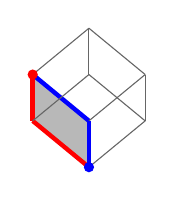
\begin{tikzpicture}%
	[x={(0.000000cm, -1.000000cm)},
	y={(1.000000cm, 0.000000cm)},
	z={(0.000000cm, 0.000000cm)},,
	scale=.5,
	back/.style={thin, color=black!60},
	edge/.style={color=black!60, thin},
	sourceedge/.style={color=red, ultra thick},
	targetedge/.style={color=blue, ultra thick},
	facet/.style={fill=black!35,fill opacity=0.800000},
	targetfacet/.style={fill=blue!80,fill opacity=0.800000},
	sourcefacet/.style={fill=red!80,fill opacity=0.800000},
	vertex/.style={inner sep=1pt,circle,draw=black,fill=black,thick},
	targetvertex/.style={inner sep=1pt,circle,draw=blue,fill=blue,thick},
	sourcevertex/.style={inner sep=1pt,circle,draw=red,fill=red,thick}]
%
\coordinate (-0.58824, 1.42857, -0.83333) at (-0.58824, 1.42857, -0.83333);
\coordinate (0.58824, 1.42857, 0.83333) at (0.58824, 1.42857, 0.83333);
\coordinate (1.76471, 0.00000, 0.00000) at (1.76471, 0.00000, 0.00000);
\coordinate (0.58824, 0.00000, -1.66667) at (0.58824, 0.00000, -1.66667);
\coordinate (-0.58824, -1.42857, -0.83333) at (-0.58824, -1.42857, -0.83333);
\coordinate (-1.76471, 0.00000, 0.00000) at (-1.76471, 0.00000, 0.00000);
\coordinate (-0.58824, 0.00000, 1.66667) at (-0.58824, 0.00000, 1.66667);
\coordinate (0.58824, -1.42857, 0.83333) at (0.58824, -1.42857, 0.83333);
%%
%%
%% Drawing edges in the back
%%

%%
%%
%% Drawing vertices in the back
%%
%%
%%
% \fill[targetfacet] (-0.58824, 0.00000, 1.66667) -- (0.58824, -1.42857, 0.83333) -- (-0.58824, -1.42857, -0.83333) -- (-1.76471, 0.00000, 0.00000) -- cycle {};
% \fill[facet] (-0.58824, 1.42857, -0.83333) -- (-1.76471, 0.00000, 0.00000) -- (-0.58824, -1.42857, -0.83333) -- (0.58824, 0.00000, -1.66667) -- cycle {};
 \fill[facet] (0.58824, 0.00000, -1.66667) -- (-0.58824, -1.42857, -0.83333) -- (0.58824, -1.42857, 0.83333) -- (1.76471, 0.00000, 0.00000) -- cycle {};


\draw[back,targetedge] (0.58824, 0.00000, -1.66667) -- (-0.58824, -1.42857, -0.83333);
\draw[edge,back] (-0.58824, -1.42857, -0.83333) -- (-1.76471, 0.00000, 0.00000);
\draw[back,sourceedge] (-0.58824, -1.42857, -0.83333) -- (0.58824, -1.42857, 0.83333);

% %% Drawing the facets
% %%
% \fill[facet] (0.58824, 0.00000, -1.66667) -- (-0.58824, 1.42857, -0.83333) -- (0.58824, 1.42857, 0.83333) -- (1.76471, 0.00000, 0.00000) -- cycle {};
% \fill[facet] (0.58824, -1.42857, 0.83333) -- (1.76471, 0.00000, 0.00000) -- (0.58824, 1.42857, 0.83333) -- (-0.58824, 0.00000, 1.66667) -- cycle {};
%  \fill[targetfacet] (-0.58824, 0.00000, 1.66667) -- (0.58824, 1.42857, 0.83333) -- (-0.58824, 1.42857, -0.83333) -- (-1.76471, 0.00000, 0.00000) -- cycle {};
%%
%%
%% Drawing edges in the front
%%
\draw[edge] (-0.58824, 1.42857, -0.83333) -- (0.58824, 1.42857, 0.83333);
\draw[edge] (-0.58824, 1.42857, -0.83333) -- (0.58824, 0.00000, -1.66667);
\draw[edge] (-0.58824, 1.42857, -0.83333) -- (-1.76471, 0.00000, 0.00000);
\draw[edge] (0.58824, 1.42857, 0.83333) -- (1.76471, 0.00000, 0.00000);
\draw[edge] (0.58824, 1.42857, 0.83333) -- (-0.58824, 0.00000, 1.66667);
\draw[targetedge] (1.76471, 0.00000, 0.00000) -- (0.58824, 0.00000, -1.66667);
\draw[sourceedge] (1.76471, 0.00000, 0.00000) -- (0.58824, -1.42857, 0.83333);
\draw[edge] (-1.76471, 0.00000, 0.00000) -- (-0.58824, 0.00000, 1.66667);
\draw[edge] (-0.58824, 0.00000, 1.66667) -- (0.58824, -1.42857, 0.83333);
%%
%%
% %% Drawing the vertices
% %%
\node[sourcevertex] at (-0.58824, -1.42857, -0.83333)     {};

% \node[vertex] at (-0.58824, 1.42857, -0.83333)     {};
% \node[targetvertex] at (0.58824, 1.42857, 0.83333)     {};
\node[targetvertex] at (1.76471, 0.00000, 0.00000)     {};
%  \node[vertex] at (0.58824, 0.00000, -1.66667)     {};
%  \node[targetvertex] at (-1.76471, 0.00000, 0.00000)     {};
% \node[vertex] at (-0.58824, 0.00000, 1.66667)     {};
% \node[vertex] at (0.58824, -1.42857, 0.83333)     {};
% %%
% %%
% %
% \begin{scope}[shift={(0,3,0)}]
%
% 		%axes
% 		\draw[->] (0, 0,0) -- (1, 0,0) node[anchor=east]{$v_1$};
% 		\draw[->] (0, 0,0) -- (0, 1,0) node[anchor=west]{$v_2$};
% 		\draw[->] (0, 0,0) -- (0, 0, 1) node[anchor=west]{$v_3$};
% 	\end{scope}

\end{tikzpicture}

\centering
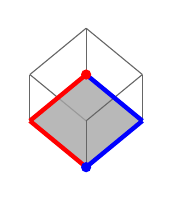
\begin{tikzpicture}%
	[x={(0.000000cm, -1.000000cm)},
	y={(1.000000cm, 0.000000cm)},
	z={(0.000000cm, 0.000000cm)},,
	scale=.5,
	back/.style={thin, color=black!60},
	edge/.style={color=black!60, thin},
	sourceedge/.style={color=red, ultra thick},
	targetedge/.style={color=blue, ultra thick},
	facet/.style={fill=black!35,fill opacity=0.800000},
	targetfacet/.style={fill=blue!80,fill opacity=0.800000},
	sourcefacet/.style={fill=red!80,fill opacity=0.800000},
	vertex/.style={inner sep=1pt,circle,draw=black,fill=black,thick},
	targetvertex/.style={inner sep=1pt,circle,draw=blue,fill=blue,thick},
	sourcevertex/.style={inner sep=1pt,circle,draw=red,fill=red,thick}]
%
\coordinate (-0.58824, 1.42857, -0.83333) at (-0.58824, 1.42857, -0.83333);
\coordinate (0.58824, 1.42857, 0.83333) at (0.58824, 1.42857, 0.83333);
\coordinate (1.76471, 0.00000, 0.00000) at (1.76471, 0.00000, 0.00000);
\coordinate (0.58824, 0.00000, -1.66667) at (0.58824, 0.00000, -1.66667);
\coordinate (-0.58824, -1.42857, -0.83333) at (-0.58824, -1.42857, -0.83333);
\coordinate (-1.76471, 0.00000, 0.00000) at (-1.76471, 0.00000, 0.00000);
\coordinate (-0.58824, 0.00000, 1.66667) at (-0.58824, 0.00000, 1.66667);
\coordinate (0.58824, -1.42857, 0.83333) at (0.58824, -1.42857, 0.83333);
%%
%%
%% Drawing edges in the back
%%

%%
%%
%% Drawing vertices in the back
%%
% \node[vertex] at (-0.58824, -1.42857, -0.83333)     {};
%%
%%
% \fill[targetfacet] (-0.58824, 0.00000, 1.66667) -- (0.58824, -1.42857, 0.83333) -- (-0.58824, -1.42857, -0.83333) -- (-1.76471, 0.00000, 0.00000) -- cycle {};
% \fill[facet] (-0.58824, 1.42857, -0.83333) -- (-1.76471, 0.00000, 0.00000) -- (-0.58824, -1.42857, -0.83333) -- (0.58824, 0.00000, -1.66667) -- cycle {};
%  \fill[facet] (0.58824, 0.00000, -1.66667) -- (-0.58824, -1.42857, -0.83333) -- (0.58824, -1.42857, 0.83333) -- (1.76471, 0.00000, 0.00000) -- cycle {};


\draw[edge,back] (0.58824, 0.00000, -1.66667) -- (-0.58824, -1.42857, -0.83333);
\draw[edge,back] (-0.58824, -1.42857, -0.83333) -- (-1.76471, 0.00000, 0.00000);
\draw[edge,back] (-0.58824, -1.42857, -0.83333) -- (0.58824, -1.42857, 0.83333);

% %% Drawing the facets
% %%
% \fill[facet] (0.58824, 0.00000, -1.66667) -- (-0.58824, 1.42857, -0.83333) -- (0.58824, 1.42857, 0.83333) -- (1.76471, 0.00000, 0.00000) -- cycle {};
\fill[facet] (0.58824, -1.42857, 0.83333) -- (1.76471, 0.00000, 0.00000) -- (0.58824, 1.42857, 0.83333) -- (-0.58824, 0.00000, 1.66667) -- cycle {};
%  \fill[targetfacet] (-0.58824, 0.00000, 1.66667) -- (0.58824, 1.42857, 0.83333) -- (-0.58824, 1.42857, -0.83333) -- (-1.76471, 0.00000, 0.00000) -- cycle {};
%%
%%
%% Drawing edges in the front
%%
\draw[edge] (-0.58824, 1.42857, -0.83333) -- (0.58824, 1.42857, 0.83333);
\draw[edge] (-0.58824, 1.42857, -0.83333) -- (0.58824, 0.00000, -1.66667);
\draw[edge] (-0.58824, 1.42857, -0.83333) -- (-1.76471, 0.00000, 0.00000);
\draw[targetedge] (0.58824, 1.42857, 0.83333) -- (1.76471, 0.00000, 0.00000);
\draw[targetedge] (0.58824, 1.42857, 0.83333) -- (-0.58824, 0.00000, 1.66667);
\draw[edge] (1.76471, 0.00000, 0.00000) -- (0.58824, 0.00000, -1.66667);
\draw[sourceedge] (1.76471, 0.00000, 0.00000) -- (0.58824, -1.42857, 0.83333);
\draw[edge] (-1.76471, 0.00000, 0.00000) -- (-0.58824, 0.00000, 1.66667);
\draw[sourceedge] (-0.58824, 0.00000, 1.66667) -- (0.58824, -1.42857, 0.83333);
%%
%%
% %% Drawing the vertices in the front
% %%
% \node[vertex] at (-0.58824, 1.42857, -0.83333)     {};
% \node[targetvertex] at (0.58824, 1.42857, 0.83333)     {};
\node[targetvertex] at (1.76471, 0.00000, 0.00000)     {};
%  \node[sourcevertex] at (0.58824, 0.00000, -1.66667)     {};
%  \node[targetvertex] at (-1.76471, 0.00000, 0.00000)     {};
 \node[sourcevertex] at (-0.58824, 0.00000, 1.66667)     {};
% \node[targetvertex] at (0.58824, -1.42857, 0.83333)     {};
% %%
% %%
% %
% \begin{scope}[shift={(0,3,0)}]
%
% 		%axes
% 		\draw[->] (0, 0,0) -- (1, 0,0) node[anchor=east]{$v_1$};
% 		\draw[->] (0, 0,0) -- (0, 1,0) node[anchor=west]{$v_2$};
% 		\draw[->] (0, 0,0) -- (0, 0, 1) node[anchor=west]{$v_3$};
% 	\end{scope}

\end{tikzpicture}
\qquad
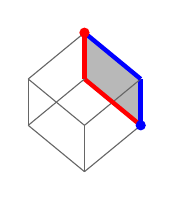
\begin{tikzpicture}%
	[x={(0.000000cm, -1.000000cm)},
	y={(1.000000cm, 0.000000cm)},
	z={(0.000000cm, 0.000000cm)},,
	scale=.5,
	back/.style={thin, color=black!60},
	edge/.style={color=black!60, thin},
	sourceedge/.style={color=red, ultra thick},
	targetedge/.style={color=blue, ultra thick},
	facet/.style={fill=black!35,fill opacity=0.800000},
	targetfacet/.style={fill=blue!80,fill opacity=0.800000},
	sourcefacet/.style={fill=red!80,fill opacity=0.800000},
	vertex/.style={inner sep=1pt,circle,draw=black,fill=black,thick},
	targetvertex/.style={inner sep=1pt,circle,draw=blue,fill=blue,thick},
	sourcevertex/.style={inner sep=1pt,circle,draw=red,fill=red,thick}]
%
\coordinate (-0.58824, 1.42857, -0.83333) at (-0.58824, 1.42857, -0.83333);
\coordinate (0.58824, 1.42857, 0.83333) at (0.58824, 1.42857, 0.83333);
\coordinate (1.76471, 0.00000, 0.00000) at (1.76471, 0.00000, 0.00000);
\coordinate (0.58824, 0.00000, -1.66667) at (0.58824, 0.00000, -1.66667);
\coordinate (-0.58824, -1.42857, -0.83333) at (-0.58824, -1.42857, -0.83333);
\coordinate (-1.76471, 0.00000, 0.00000) at (-1.76471, 0.00000, 0.00000);
\coordinate (-0.58824, 0.00000, 1.66667) at (-0.58824, 0.00000, 1.66667);
\coordinate (0.58824, -1.42857, 0.83333) at (0.58824, -1.42857, 0.83333);
%%
%%
%% Drawing edges in the back
%%

%%
%%
%% Drawing vertices in the back
%%
% \node[vertex] at (-0.58824, -1.42857, -0.83333)     {};
%%
%%
% \fill[targetfacet] (-0.58824, 0.00000, 1.66667) -- (0.58824, -1.42857, 0.83333) -- (-0.58824, -1.42857, -0.83333) -- (-1.76471, 0.00000, 0.00000) -- cycle {};
% \fill[facet] (-0.58824, 1.42857, -0.83333) -- (-1.76471, 0.00000, 0.00000) -- (-0.58824, -1.42857, -0.83333) -- (0.58824, 0.00000, -1.66667) -- cycle {};
%  \fill[facet] (0.58824, 0.00000, -1.66667) -- (-0.58824, -1.42857, -0.83333) -- (0.58824, -1.42857, 0.83333) -- (1.76471, 0.00000, 0.00000) -- cycle {};


\draw[edge,back] (0.58824, 0.00000, -1.66667) -- (-0.58824, -1.42857, -0.83333);
\draw[edge,back] (-0.58824, -1.42857, -0.83333) -- (-1.76471, 0.00000, 0.00000);
\draw[edge,back] (-0.58824, -1.42857, -0.83333) -- (0.58824, -1.42857, 0.83333);

% %% Drawing the facets
% %%
% \fill[facet] (0.58824, 0.00000, -1.66667) -- (-0.58824, 1.42857, -0.83333) -- (0.58824, 1.42857, 0.83333) -- (1.76471, 0.00000, 0.00000) -- cycle {};
% \fill[facet] (0.58824, -1.42857, 0.83333) -- (1.76471, 0.00000, 0.00000) -- (0.58824, 1.42857, 0.83333) -- (-0.58824, 0.00000, 1.66667) -- cycle {};
 \fill[facet] (-0.58824, 0.00000, 1.66667) -- (0.58824, 1.42857, 0.83333) -- (-0.58824, 1.42857, -0.83333) -- (-1.76471, 0.00000, 0.00000) -- cycle {};
%%
%%
%% Drawing edges in the front
%%
\draw[targetedge] (-0.58824, 1.42857, -0.83333) -- (0.58824, 1.42857, 0.83333);
\draw[edge] (-0.58824, 1.42857, -0.83333) -- (0.58824, 0.00000, -1.66667);
\draw[targetedge] (-0.58824, 1.42857, -0.83333) -- (-1.76471, 0.00000, 0.00000);
\draw[edge] (0.58824, 1.42857, 0.83333) -- (1.76471, 0.00000, 0.00000);
\draw[sourceedge] (0.58824, 1.42857, 0.83333) -- (-0.58824, 0.00000, 1.66667);
\draw[edge] (1.76471, 0.00000, 0.00000) -- (0.58824, 0.00000, -1.66667);
\draw[edge] (1.76471, 0.00000, 0.00000) -- (0.58824, -1.42857, 0.83333);
\draw[sourceedge] (-1.76471, 0.00000, 0.00000) -- (-0.58824, 0.00000, 1.66667);
\draw[edge] (-0.58824, 0.00000, 1.66667) -- (0.58824, -1.42857, 0.83333);
%%
%%
% %% Drawing the vertices in the front
% %%
% \node[sourcevertex] at (-0.58824, 1.42857, -0.83333)     {};
\node[targetvertex] at (0.58824, 1.42857, 0.83333)     {};
% \node[sourcevertex] at (1.76471, 0.00000, 0.00000)     {};
%  \node[sourcevertex] at (0.58824, 0.00000, -1.66667)     {};
 \node[sourcevertex] at (-1.76471, 0.00000, 0.00000)     {};
%  \node[targetvertex] at (-0.58824, 0.00000, 1.66667)     {};
% \node[targetvertex] at (0.58824, -1.42857, 0.83333)     {};
% %%
% %%
% %
% \begin{scope}[shift={(0,3,0)}]
%
% 		%axes
% 		\draw[->] (0, 0,0) -- (1, 0,0) node[anchor=east]{$v_1$};
% 		\draw[->] (0, 0,0) -- (0, 1,0) node[anchor=west]{$v_2$};
% 		\draw[->] (0, 0,0) -- (0, 0, 1) node[anchor=west]{$v_3$};
% 	\end{scope}

\end{tikzpicture}
\qquad
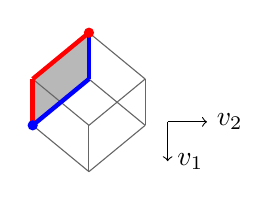
\begin{tikzpicture}%
	[x={(0.000000cm, -1.000000cm)},
	y={(1.000000cm, 0.000000cm)},
	z={(0.000000cm, 0.000000cm)},,
	scale=.5,
	back/.style={thin, color=black!60},
	edge/.style={color=black!60, thin},
	sourceedge/.style={color=red, ultra thick},
	targetedge/.style={color=blue, ultra thick},
	facet/.style={fill=black!35,fill opacity=0.800000},
	targetfacet/.style={fill=blue!80,fill opacity=0.800000},
	sourcefacet/.style={fill=red!80,fill opacity=0.800000},
	vertex/.style={inner sep=1pt,circle,draw=black,fill=black,thick},
	targetvertex/.style={inner sep=1pt,circle,draw=blue,fill=blue,thick},
	sourcevertex/.style={inner sep=1pt,circle,draw=red,fill=red,thick}]
%
\coordinate (-0.58824, 1.42857, -0.83333) at (-0.58824, 1.42857, -0.83333);
\coordinate (0.58824, 1.42857, 0.83333) at (0.58824, 1.42857, 0.83333);
\coordinate (1.76471, 0.00000, 0.00000) at (1.76471, 0.00000, 0.00000);
\coordinate (0.58824, 0.00000, -1.66667) at (0.58824, 0.00000, -1.66667);
\coordinate (-0.58824, -1.42857, -0.83333) at (-0.58824, -1.42857, -0.83333);
\coordinate (-1.76471, 0.00000, 0.00000) at (-1.76471, 0.00000, 0.00000);
\coordinate (-0.58824, 0.00000, 1.66667) at (-0.58824, 0.00000, 1.66667);
\coordinate (0.58824, -1.42857, 0.83333) at (0.58824, -1.42857, 0.83333);
%%
%%
%% Drawing edges in the back
%%

%%
%%
%% Drawing vertices in the back
%%
%%
%%
\fill[facet] (-0.58824, 0.00000, 1.66667) -- (0.58824, -1.42857, 0.83333) -- (-0.58824, -1.42857, -0.83333) -- (-1.76471, 0.00000, 0.00000) -- cycle {};
% \fill[facet] (-0.58824, 1.42857, -0.83333) -- (-1.76471, 0.00000, 0.00000) -- (-0.58824, -1.42857, -0.83333) -- (0.58824, 0.00000, -1.66667) -- cycle {};
%  \fill[facet] (0.58824, 0.00000, -1.66667) -- (-0.58824, -1.42857, -0.83333) -- (0.58824, -1.42857, 0.83333) -- (1.76471, 0.00000, 0.00000) -- cycle {};


\draw[edge,back] (0.58824, 0.00000, -1.66667) -- (-0.58824, -1.42857, -0.83333);
\draw[back,sourceedge] (-0.58824, -1.42857, -0.83333) -- (-1.76471, 0.00000, 0.00000);
\draw[back,sourceedge] (-0.58824, -1.42857, -0.83333) -- (0.58824, -1.42857, 0.83333);

% %% Drawing the facets
% %%
% \fill[facet] (0.58824, 0.00000, -1.66667) -- (-0.58824, 1.42857, -0.83333) -- (0.58824, 1.42857, 0.83333) -- (1.76471, 0.00000, 0.00000) -- cycle {};
% \fill[facet] (0.58824, -1.42857, 0.83333) -- (1.76471, 0.00000, 0.00000) -- (0.58824, 1.42857, 0.83333) -- (-0.58824, 0.00000, 1.66667) -- cycle {};
%  \fill[facet] (-0.58824, 0.00000, 1.66667) -- (0.58824, 1.42857, 0.83333) -- (-0.58824, 1.42857, -0.83333) -- (-1.76471, 0.00000, 0.00000) -- cycle {};
%%
%%
%% Drawing edges in the front
%%
\draw[edge] (-0.58824, 1.42857, -0.83333) -- (0.58824, 1.42857, 0.83333);
\draw[edge] (-0.58824, 1.42857, -0.83333) -- (0.58824, 0.00000, -1.66667);
\draw[edge] (-0.58824, 1.42857, -0.83333) -- (-1.76471, 0.00000, 0.00000);
\draw[edge] (0.58824, 1.42857, 0.83333) -- (1.76471, 0.00000, 0.00000);
\draw[edge] (0.58824, 1.42857, 0.83333) -- (-0.58824, 0.00000, 1.66667);
\draw[edge] (1.76471, 0.00000, 0.00000) -- (0.58824, 0.00000, -1.66667);
\draw[edge] (1.76471, 0.00000, 0.00000) -- (0.58824, -1.42857, 0.83333);
\draw[targetedge] (-1.76471, 0.00000, 0.00000) -- (-0.58824, 0.00000, 1.66667);
\draw[targetedge] (-0.58824, 0.00000, 1.66667) -- (0.58824, -1.42857, 0.83333);
%%
%%
% %% Drawing the vertices

% \node[targetvertex] at (-0.58824, -1.42857, -0.83333)     {};

% %%
% \node[sourcevertex] at (-0.58824, 1.42857, -0.83333)     {};
% \node[targetvertex] at (0.58824, 1.42857, 0.83333)     {};
% \node[sourcevertex] at (1.76471, 0.00000, 0.00000)     {};
%  \node[sourcevertex] at (0.58824, 0.00000, -1.66667)     {};
 \node[sourcevertex] at (-1.76471, 0.00000, 0.00000)     {};
%  \node[sourcevertex] at (-0.58824, 0.00000, 1.66667)     {};
 \node[targetvertex] at (0.58824, -1.42857, 0.83333)     {};
% %%
% %%
% %
% \begin{scope}[shift={(0,3,0)}]
%
% 		%axes
% 		\draw[->] (0, 0,0) -- (1, 0,0) node[anchor=east]{$v_1$};
% 		\draw[->] (0, 0,0) -- (0, 1,0) node[anchor=west]{$v_2$};
% 		\draw[->] (0, 0,0) -- (0, 0, 1) node[anchor=west]{$v_3$};
% 	\end{scope}
\begin{scope}[shift={(.5,2,0)}]
	\draw[->] (0, 0,0) -- (1, 0,0) node[anchor=west]{$v_1$};
	\draw[->] (0, 0,0) -- (0, 1,0) node[anchor=west]{$v_2$};
\end{scope}
\end{tikzpicture}
\\ \ \par
\end{frame}

\begin{frame}{Sources and targets}

	Let $P$ be framed by $\{v_i\}$ and $F \in \faces(P)$.

	\medskip
	For $k < \dim F$, the \colorit{$k$-boundary} $\bd^{(k)}(F)$ is the boundary of $\pi_{k+1}(F)$.

	\smallskip
	It has a canonical splitting:
	\[
	\bd^{(k)}(F) = \colorit{\so_k(F)} \sqcup \colorit{\ta_k(F)}
	\]
	where these are defined using the normal
	\[
	\angles{\normal, v_{k+1}} < 0 \quad (\text{resp.} > 0).
	\]
	\pause\medskip
	\colorit{Example} ...

	\pause\bigskip
	\colorit{Claim} The moduli of frames over these so/ta splittings is also universal.

	\pause\bigskip
	\colorit{Reason} Orientations double cover these so/ta splittings.
\end{frame}

\begin{frame}{Digression (for computational geometers)}
	\pause
	This double cover is analogous to that of chirotopes over oriented matroids.

	\pause\medskip
	For simplices, we constructed a bijection between:

	\medskip
	$\bullet$ \colorit{frame orientations} \& (uniform and acyclic) \colorit{realizable flag chirotopes}

	\pause\medskip
	$\bullet$ \colorit{so/ta splitting structures} \& (...) \colorit{flag oriented matroids}.

	\pause\bigskip
	\colorit{Disclaimer} This will play no role today.

	\pause\medskip
	Let us go back to the idea of Kapranov-Voevodsky, again.
\end{frame}

\begin{frame}{Strings and loops}
	\pause
	A \colorit{$k$-string} in $P$ is a tuple $(F_1,\dots,F_\ell)$ of faces with
	\[
	\ta_k(F_i) \cap \so_k(F_{i+1}) \neq \emptyset.
	\]

	\pause
	\colorit{Claim} This intersection is always a single $k$-face.

	\pause\medskip
	\colorit{Example} TBA3

	\pause\medskip
	We say it is a \colorit{$k$-loop} if $F_i = F_j$ for some $i \neq j$.

	\pause\medskip
	\colorit{Claim}
	There are no $0$-loops on any framed polytope.
	\pause
	\begin{enumerate}
		\item We can replace the frame for an orthogonal one.
		\item $\angles{-, v_1}$ is strictly increasing over the string.
	\end{enumerate}

	\pause\medskip
	\colorit{Theorem} A framed polytope defines a pasting diagram iff it is loop-free.

	\pause\medskip
	\colorit{Comment} We used Steiner's theory of directed complexes.

	\pause\medskip
	\colorit{Question} Are there $k$-loops?

\end{frame}

\begin{frame}{A 1-loop of 2-faces in the 5-simplex}
	\pause
	Consider $p_1,\dots,p_6 \in \R^5$
	\[
	\begin{pmatrix}
		-3 \\
		-1 \\
		-1 \\
		0 \\
		1
	\end{pmatrix}
	\begin{pmatrix}
		-2 \\
		1 \\
		1 \\
		0 \\
		1
	\end{pmatrix}
	\begin{pmatrix}
		-1 \\
		0 \\
		0 \\
		1 \\
		1
	\end{pmatrix}
	\begin{pmatrix}
		1 \\
		0 \\
		0 \\
		1 \\
		0
	\end{pmatrix}
	\begin{pmatrix}
		2 \\
		1 \\
		-1 \\
		0 \\
		0
	\end{pmatrix}
	\begin{pmatrix}
		3 \\
		-1 \\
		1 \\
		0 \\
		0
	\end{pmatrix}
	\]
	They form a $5$-simplex $P$ and the canonical frame is $P$-admissible.

	\pause\medskip

	\resizebox{\linewidth}{!}{
		\begin{tikzpicture}[auto, node distance=2cm, >=latex',
			point/.style = {draw, circle, fill = black, inner sep = 1pt}]

			\coordinate (a) at (-3,-1);
			\coordinate (b) at (-2,1);
			\coordinate (c) at (-1,0);
			\coordinate (d) at (1,0);
			\coordinate (e) at (2,1);
			\coordinate (f) at (3,-1);

			\draw[thick] (c) -- (f) -- (b) -- (d);
			\draw[line width = 3pt,white] (d) -- (a) -- (e) -- (c);
			\draw[thick] (d) -- (a) -- (e) -- (c);
			\draw[thick] (a) -- (b) -- (c) -- (a);
			\draw[thick] (d) -- (e) -- (f) -- (d);

			\foreach \i/\l in {a/p_1,b/p_2,c/p_3,d/p_4,e/p_5,f/p_6}
			{
				\node[point,label={above:$\l$}] at (\i) {};
			}

			\draw[->] (4,0)-- (4,1);
			\draw[->] (4,0)-- (5,0);
			\node[] at (5.5, 0) {$e_1$};
			\node[] at (4.5, 1) {$e_2$};
	\end{tikzpicture}}
\end{frame}

\begin{frame}{The cyclic $n$-simplex}
	\pause
	Is the convex closure of
	\[
	\set[\big]{(t,t^2,\dots,t^n) \mid t \in \{0,\dots,n-1\}}.
	\]

	\pause
	\colorit{Theorem}

	\smallskip
	With the canonical frame $\{e_1,e_2,\dots\}$ the cyclic simplex is loop free.

	\pause\smallskip
	Additionally, with $\{e_1,-e_2,e_3,-e_4,\dots\}$ it exactly recovers Street's pasting diagrams.
\end{frame}

\begin{frame}{How special is this embedding}
	\pause
	A \colorit{Gaussian $n$-simplex} as the convex hull of $n+1$ independent random points in~$\R^n$ each chosen according to a $n$-dim'l std. normal distribution.

	\pause\medskip
	\colorit{Theorem (LPM)} The probability that a canonically framed Gaussian $n$-simplex has a loop tends to~$1$ as~$n$ tends to~$\infty$.

	\pause\medskip
	\colorit{Slogan} Loop-free framed polytopes are special.
\end{frame}

\begin{frame}{Summary}
	\pause
	\begin{enumerate}
		\item\pause Framed and oriented polytopes.
		\item\pause The moduli of frames over an orientation can be wild.
		\item\pause Kapranov-Voevodsky conjecture (KVC):

		\smallskip
		Framed $n$-polytopes define $n$-categorical pasting diagrams.

		\item\pause Main example:

		\smallskip
		Cyclic $n$-simplex defines Street's pasting diagrams.

		\item\pause KVC is equivalent to loop-freeness.

		\item\pause First counterexample: a 1-loop of 2-faces in a 5-simplex.

		\item\pause Loop-freeness is vanishingly rare (in a precise sense).

		\item\pause Future work:

		\smallskip
		Flags of oriented matroids instead of framed polytopes.
	\end{enumerate}
\end{frame}

%\begin{frame}{Oriented posets}
%	\pause
%	Let $(\Gamma, \leq)$ be a poset and $z \in \Gamma$.
%	The \colorit{cover set} of $z$:
%	\[
%	\cov(z) = \set{x < z \mid \nexists y,\ x < y < z}.
%	\]
%
%	\pause
%	An \colorit{orientation} is a partition $\so(z) \sqcup \ta(z) = \cov(z)$ for each $z \in P$.
%
%	\pause\bigskip
%	\colorit{Construction} An orientation $\omega$ of $P$ induces an orientation on $\faces(P)$.
%
%	\pause
%	\[
%	\text{Facet } E \leq F \text{ in } \ta(F) \qquad iff \qquad \omega_F \sim (\normal_E^F \wedge \, \omega_E).
%	\]
%
%	\pause\bigskip
%	\colorit{Ambiguity} This orientation on $\faces(P)$ determines $\omega$ up to
%	\[
%	\forall F,\ \omega_F \mapsto - \omega_F.
%	\]
%\end{frame}
%
%\begin{frame}{Refinement systems}
%	\pause
%	A \colorit{poset refinement system} is a collection $\set{\leq_i}$ of poset relations on $X$~s.t.
%	\[
%	\id \colon (X, \leq_i) \to (X, \leq_j)
%	\]
%	is order-preserving for $i \leq j$.
%
%	\pause\medskip
%	\colorit{Construction} If $P$ is framed then $\faces(P)$ has a poset refinement system.
%
%	\pause
%	\[
%	F \leq_k G \qquad iff \qquad \pi_k(F) \subseteq \pi_k(G)
%	\]
%
%	\pause\smallskip
%	Each poset $(\faces(P), \leq_k)$ has a canonical orientation induced by the frame.
%	\[
%	\pi_k(F),
%	\]
%
%	\pause\medskip
%	For $F \in \faces(P)$ say $\dim f = m$, then $k$-source and $k$-target of $F \in \faces(P)$
%	\[
%	\so_k(F) = {}
%	\]
%
%\end{frame}
